\section{Scrum}

O Scrum é um \textit{framework} de desenvolvimento ágil que consiste em um time, suas atividades associadas, artefatos e regras que servem para entregar uma série de incrementos de produto dentro de um determinado período (geralmente de 2 a 4 semanas) chamado \textit{sprint} \cite{livro-scrum}.
O time é formado por:
\begin{itemize}
\item \textbf{\textit{Product Owner}}, responsável por manter os requisitos e dividí-los para o resto da equipe \cite{product-owner};
\item \textbf{\textit{Scrum Master}}, responsável por liderar e ajudar a equipe de desenvolvimento, ser a ponte entre o \textit{product owner} e a equipe para conduzir as reuniões mantendo a sincronia do projeto \cite{scrum-master};
\item \textbf{Equipe de desenvolvimento}, profissionais responsáveis por desenvolver o produto e entregá-lo ao fim de cada \textit{sprint} \cite{equipe-dev}.
\end{itemize}

O Scrum começa com a visão do \textit{product owner} sobre o produto e a criação das funcionalidades do sistema em uma lista priorizada chamada \textit{product backlog}. Depois, são separadas tarefas do \textit{backlog} para compor a \textit{sprint}, de acordo com o que a equipe acredita conseguir desenvolver durante o ciclo, e assim a \textit{sprint} se inicia. No final, é feita uma revisão da \textit{sprint}, onde os itens desenvolvidos pela equipe são revisados por todos as partes envolvidas, e é feita uma retrospectiva, que mostra os pontos positivos e negativos da \textit{sprint}, a fim de melhorar a próxima \cite{livro-scrum}. A Figura \ref{img:scrum} mostra o fluxo das atividades do Scrum.

\begin{figure}[H]
    \centering
    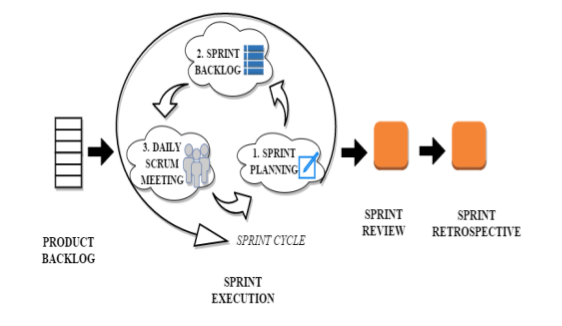
\includegraphics[scale=0.5]{figuras/scrum.png}
    \caption[Fluxograma do Scrum]{Fluxograma do Scrum. Fonte: \cite{artigo-scrum}}
    \label{img:scrum}
\end{figure}
